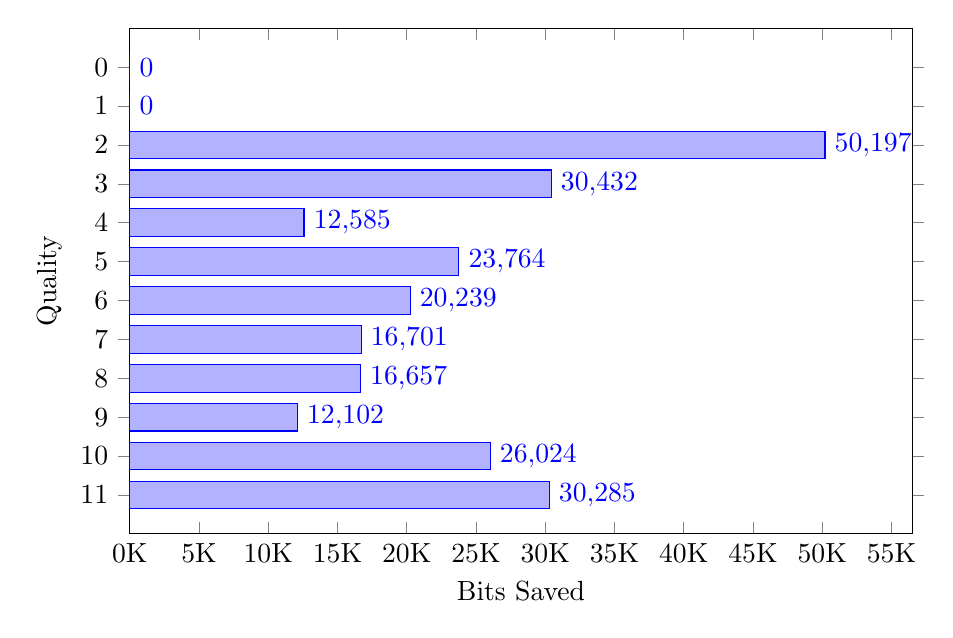
\begin{tikzpicture}
\begin{axis}[
	width = 0.95\textwidth,
	height = 1.1*\axisdefaultheight,
	xbar,
	xmax = 56500,
	xtick = {0, 5000, 10000, 15000, 20000, 25000, 30000, 35000, 40000, 45000, 50000, 55000},
	xticklabels = {$0$K, $5$K, $10$K, $15$K, $20$K, $25$K, $30$K, $35$K, $40$K, $45$K, $50$K, $55$K},
	y dir = reverse,
	ytick = data,
	scaled ticks = false,
	enlarge x limits = {abs = 0},
	enlarge y limits = {abs = 1},
	nodes near coords,
	nodes near coords align = {horizontal},
	xlabel = Bits Saved,
	ylabel = Quality
]
\addplot coordinates {
	(0, 0)
	(0, 1)
	(50197, 2)
	(30432, 3)
	(12585, 4)
	(23764, 5)
	(20239, 6)
	(16701, 7)
	(16657, 8)
	(12102, 9)
	(26024, 10)
	(30285, 11)
};
\end{axis}
\end{tikzpicture}